%%%%%%%%%%%%%%%%%%%%%%%%%%%%%%%%%%%%%%%%%
% Journal Article
% LaTeX Template
% Version 1.3 (9/9/13)
%
% This template has been downloaded from:
% http://www.LaTeXTemplates.com
%
% Original author:
% Frits Wenneker (http://www.howtotex.com)
%
% License:
% CC BY-NC-SA 3.0 (http://creativecommons.org/licenses/by-nc-sa/3.0/)
%
%%%%%%%%%%%%%%%%%%%%%%%%%%%%%%%%%%%%%%%%%

%----------------------------------------------------------------------------------------
%	PACKAGES AND OTHER DOCUMENT CONFIGURATIONS
%----------------------------------------------------------------------------------------

\documentclass[twoside]{article}

\usepackage{lipsum} % Package to generate dummy text throughout this template

\usepackage[sc]{mathpazo} % Use the Palatino font
\usepackage[T1]{fontenc} % Use 8-bit encoding that has 256 glyphs
\linespread{1.05} % Line spacing - Palatino needs more space between lines
\usepackage{microtype} % Slightly tweak font spacing for aesthetics

\usepackage[hmarginratio=1:1,top=32mm,columnsep=20pt]{geometry} % Document margins
\usepackage{multicol} % Used for the two-column layout of the document
\usepackage[hang, small,labelfont=bf,up,textfont=it,up]{caption} % Custom captions under/above floats in tables or figures
\usepackage{booktabs} % Horizontal rules in tables
\usepackage{float} % Required for tables and figures in the multi-column environment - they need to be placed in specific locations with the [H] (e.g. \begin{table}[H])
\usepackage{hyperref} % For hyperlinks in the PDF

\usepackage{lettrine} % The lettrine is the first enlarged letter at the beginning of the text
\usepackage{paralist} % Used for the compactitem environment which makes bullet points with less space between them

\usepackage{abstract} % Allows abstract customization
\renewcommand{\abstractnamefont}{\normalfont\bfseries} % Set the "Abstract" text to bold
\renewcommand{\abstracttextfont}{\normalfont\small\itshape} % Set the abstract itself to small italic text

\usepackage{titlesec} % Allows customization of titles
\renewcommand\thesection{\Roman{section}} % Roman numerals for the sections
\renewcommand\thesubsection{\Roman{subsection}} % Roman numerals for subsections
\titleformat{\section}[block]{\large\scshape\centering}{\thesection.}{1em}{} % Change the look of the section titles
\titleformat{\subsection}[block]{\large}{\thesubsection.}{1em}{} % Change the look of the section titles

\usepackage{fancyhdr} % Headers and footers
\pagestyle{fancy} % All pages have headers and footers
\fancyhead{} % Blank out the default header
\fancyfoot{} % Blank out the default footer
\fancyfoot[RO,LE]{\thepage} % Custom footer text

%----------------------------------------------------------------------------------------
%	TITLE SECTION
%----------------------------------------------------------------------------------------

\title{\vspace{-15mm}\fontsize{24pt}{10pt}\selectfont\textbf{Super Awesome Wikipedia Hops Fairness Article}} % Article title
\author{
\large
\textsc{Blandine Seznec}\\[2mm] % Your name
\normalsize \href{mailto:Blandine@seznec.com}{blandine@seznec.com} % Your email address
\and
\textsc{Philip Thruesen }\\[2mm] % Your name
\normalsize \href{mailto:Philip@thruesen.com}{Philip@thruesen.com} % Your email address
\and
\textsc{Patrick Bach Andersen}\\[2mm] % Your name
\normalsize \href{mailto:Philip@thruesen.com}{Philip@thruesen.com} % Your email address
\and
\textsc{Jaroslav Cechak}\\[2mm] % Your name
\normalsize \href{mailto:Jaroslav@cechak.com}{Jaroslav@cechak.com} % Your email address
\and
\textsc{Roel Castano}\\[2mm] % Your name
\normalsize \href{mailto:Roel@castano.com}{Roel@castano.com} % Your email address
}
\date{}

%----------------------------------------------------------------------------------------

\begin{document}

\maketitle % Insert title

\thispagestyle{fancy} % All pages have headers and footers


% Abstract
\begin{abstract}

\noindent \lipsum[1] % Dummy abstract text


This paper explores the user behaviour in 
\end{abstract}


%----------------------------------------------------------------------------------------
%	ARTICLE CONTENTS
%----------------------------------------------------------------------------------------

\begin{multicols}{2} % Two-column layout throughout the main article text

\section{Introduction}

As technology becomes part of all aspects of human nature and new trends such as the internet of things connect everyday objects to the internet, the amount of data stored in the digital universe has been growing at an outstanding rate. Consequently, processing and analysing data sets has become increasingly difficult and techniques have been developed in the fields of machine learning, big data, and others to facilitate the use of data. \\
One of the many problems that arises from this growth of digital capacity is information retrieval. We can see examples of this with search engines, recommender systems, bioinformatics, and many more, where it is necessary to rank data sets based on relevance to a certain query taking into account multiple features which influence the relevance of each option. For cases like this ones, algorithms like Learning to Rank \\
One interesting case where Learning to Rank (L2R) could be applied is to extract the importance of links in Wikipedia articles to prevent Overlinking; Containing excessive number of links, making it difficult to likely to aid the user \cite{missing_links}. Wikipedia is an internet encyclopaedia with more than 38 million articles in over 250 different languages of semi-structured information. It is also the most popular wiki-based website, and is ranked by Alexa as the \#6 most popular website in the internet. It allows the collaborative modification of its articles by the users, which is one of the main reasons Wikipedia has grown to such an impressive size. \\
Being ``the free encyclopedia that anyone can edit'' has many advantages and disadvantages, and one of the disadvantages is, as mentioned before, Overlinking. As mentioned in a study by Ashwin Paranjape et al. \cite{paranjape}:  ``in the English Wikipedia, of all the 800,000 links added ... in February 2015, the majority (66\%) were not clicked even a single time in March 2015, and among the rest, most links were clicked only very rarely''. Since most of the editing of articles is done manually, finding and removing useless links to other articles is hard to do and editors do not focus on this. Given this case, we would like answer the following questions.

\begin{itemize}
\item Is it possible reduce the amount of links in Wikipedia articles by ranking the most relevant links based on a set of the most important features?
\item How could the features for the L2R algorithm be chosen for maximum effectiveness?
\item Will reducing the number of links in a Wikipedia article improve the readability of an article and aid the reader in finding interesting and relevant links?
\end{itemize}


%------------------------------------------------

\subsection{Related Work}
\subsubsection*{Learning to Rank Approach}
Previous work has been done in determining value of content in social networks by utilizing L2R algorithms. Similar work was done by Duan et. al. \cite{l2rtwitter}, who worked in analyzing micro-blogging systems, focusing on the Twitter social network, and extracting features which could impact the relevance of a tweet. 

\subsubsection*{Wikipedia}
Another already explored area is the link structure in Wikipedia, from which we acquired key concepts for this article. \cite{learning_link} explores the issue of disambiguation and detection of possible links in external texts. In addition to the main focus in automatic cross-reference of external articles, this paper provides an understanding of certain techniques used to detect potential links in articles and the proper reference (disambiguation) of terms in Wikipedia. Detecting links relies in a machine learning algorithm similar to the one applied in this article which weights in different features of the articles to provide a score to all potential links and choose the final ones. Examples of features used in this implementation include link probability, relatedness of topics, disambiguation confidence, and many others.  Learning to disambiguate links on the other hand, means identifying the correct meaning, for example ``crane'', as a large bird or a mechanical lifting machine, depending on the context (using unambiguous concepts for example) and probability of said word.

On the other hand, West et. al. \cite{west} add on the topic of identifying missing hyperlinks by utilizing datasets of navigation paths from Wikipedia-based games in which users try to find the shortest paths between articles, which is useful for understanding user navigation. They then\cite{paranjape}  point out missing references by making use of server logs to weight the usefulness of links that don't exist yet. By studying the user's paths through Wikipedia, they find patterns which could be shortened with missing links.

%------------------------------------------------

\section{Learning to Rank Algorithm}

The algorithm used for choosing from the list of links is called Learning to Rank. This machine learning algorithm ranks a set of 'documents' given a query based on a set of features defined previously and provides a label (grade) to these documents. The label, or relevance of a document, can be given in multiple forms:

\begin{itemize}  
\item Binary Label 
\item Multi-Level Judgement 
\item Pairwise Preferences 
\end{itemize}



%------------------------------------------------

\section{Features}
This section defines each feature used in the implementation of Learn to Rank algorithm.

\subsection{Link Position}
\subsubsection{Description}
Position of a link in an article is the number of characters counted from the beginning of the article up to the link appearance. Because the length of different articles may vary quite substantially, this number is normalized per article.

\subsubsection{Motivation}
Our intuition behind the Link Position feature is based on two observations. The first one is that given the way Wikipedia articles are structured, the most general description of the article is placed in the first few paragraphs before the table of contents. This section of the Wikipedia article is called the lead \cite{lead}. As described in the Wikipedia manual of style, for many people, the lead section is the only section they will read since it summarises the entire article. Later paragraphs only dive deeper into the topics outlined in the description. 

The second observation is the way people read web pages. As explained in \cite{nielsen} by Jakob Nielsen, one of the leaders in human-computer interaction, on average, users have time to read at most 28 \% of the words on a website. Additionally, most attention is given to the top portion of a page and later sections are merely skimmed through. People looking for different article that is somewhat related to the one currently being read might be interested in more general concepts as they contain the searched term. As explained above, more general terms happen to be heavily abundant in the top portion of a Wikipedia article.

\subsubsection{Extraction}
Raw texts of the articles in Wiki markup are taken from the Wikipedia dumps described above and links to other articles are found using regular expressions. Links to images, external sources, etc. are ignored. Due to the nature of source, from which is this feature extracted, there might be slight discrepancies in position value and the exact number of characters preceding the links in final article as displays in web browser.

\subsection{Link Order}

\subsubsection{Description}
This feature captures the position of link relative to all the other links contained in the same article. The order equal to $n$ means that the link is the $n^{th}$ link in the article. The final value of this feature is again normalised per article.

\subsubsection{Motivation}
Similar to the previous feature, Link Order is based on the observation that a Wikipedia article's initially describe the topic in general terms. While the link position captures more of a distance between links and their spread, link order is a simplified version of it. It conveys less information, but in a much more straightforward manner.

\subsubsection{Extraction}
This feature is also extracted from the Wikipedia dumps in a similar manner to the Link Position feature.

\subsection{Link Count}

\subsubsection{Description}
Link Count is the number of occurrences of the same link throughout the article.

\subsubsection{Motivation}
Whenever a link is present multiple times in a single article, it means that the topic is repeated several times in the article as well. This may signify strong relatedness of articles content.

\subsubsection{Extraction}
The feature is extracted from the Wikipedia dump using the raw article texts as in case of the previous two features.


\subsection{Community Membership}

\subsubsection{Description}
Let $G(V,E)$ be a simple graph. Then a community in $G$ is a subgraph $(V', E') = G' \subseteq G$, such that $|E'| \ge |\{ \{u,v\} \in E\setminus E'  \; | \; \{u, v\} \cap V' \neq \emptyset \}|$. In our case the $G$ is a graph of Wikipedia, where $V$ is a set of articles and $E$ is set of links between them. After detecting all communities, each edge (link) $\{u,v\}$ is given a value of 1 if both vertices belong to the same community or -1 otherwise.

\subsubsection{Motivation}
Communities are an implicit clustering of articles on Wikipedia that capture emerging properties of interconnected articles. This feature looks promising in cases where someone is interested in a specific topic, be it music bands of the same genre or fields of study in a certain science. Related articles from the same community might be a good place to look at and will highly likely contain desired article. Furthermore, users reading an article have shown an interest in specific topic and might want to broaden and deepen his or her knowledge of it.

\subsubsection{Extraction}
Every link extracted from the Wikipedia dump is converted into an edge of a graph. The resulting graph is then loaded and communities are found using igraph package in R. Community detection algorithms used were \cite{fast_greedy}, \cite{label_propagation}, and \cite{infomap}. The graph was transformed into a simple graph and then community detection algorithms were run. Even though links have natural orientation, one can relax them as undirected edges. Sheer number of links by it self is an adequate indicator of community belonging regardless of their orientation.

\subsection{Symmetric Linking}
This feature captures the notion of two article being interconnected in both directions. Formally, a link $(A,B)$ between article A and B is symmetric if and only if link $(B,A)$ also exists. Symmetric linking indicates, in some cases, that there exists an important relevance between said articles or highly related topics are being discussed. Examples of this article relationship includes competing presidential candidates, sports team rivals, movies and its actors, etc. As expected, it is common for users to demonstrate interest in these kind of relations between articles. By looking and the article relationships, we found in one sample of the most visited articles that 74.9\% of the links were non-symmetric and 25.1\% were symmetric.

\subsection{HITS and PageRanks}

Although HITS and PageRank differ in content their main goal is the same, give estimate of article significance. In case of HITS, high hub score may indicate more general topics while high authority score would be indication of very focused article discussing particular term in great depth. PageRank is similar to the hub and authority score combined. \\

Similarly to community extraction, HITS and PageRank are computed from graph representation of Wikipedia. The graph is processed in R using package igraph that implements both scores. \\

The intuition behind this feature comes from the search engine domain. In search, these scores helps identify the most relevant results. When applied to articles, the scores will help categorise linked articles for the learning to rank algorithm.


%------------------------------------------------

% slide 29: visualize results in bar chart. Select important algos and have 4 bars (each of eval. methods)
% slide xx: some more slides with e.g. zeros..
% slide xx: examples of ranking

\begin{frame}
  \frametitle{Results for NDCG@10}
  \begin{figure}[tbph]
    \centering
    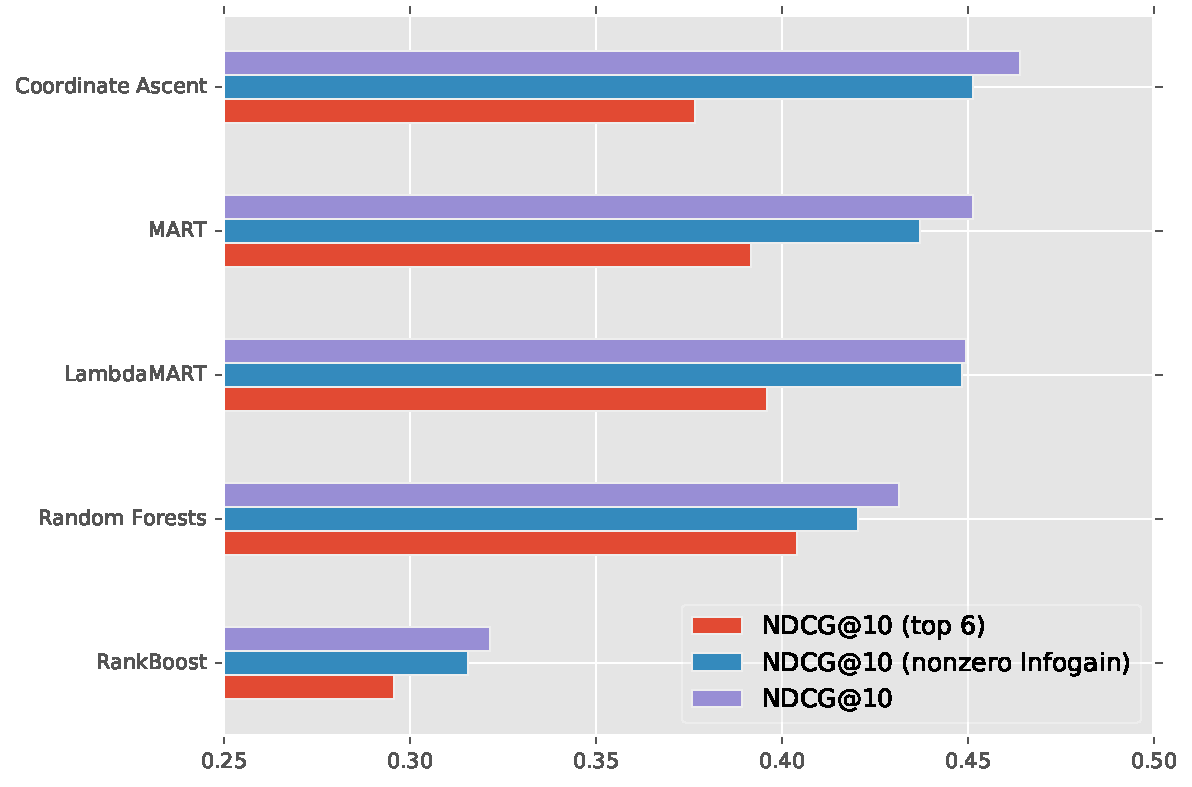
\includegraphics[width=\linewidth]{images/results_ndcg10}
  \end{figure}
\end{frame}

\begin{frame}
  \frametitle{Results for P@191}
  \begin{figure}[tbph]
    \centering
    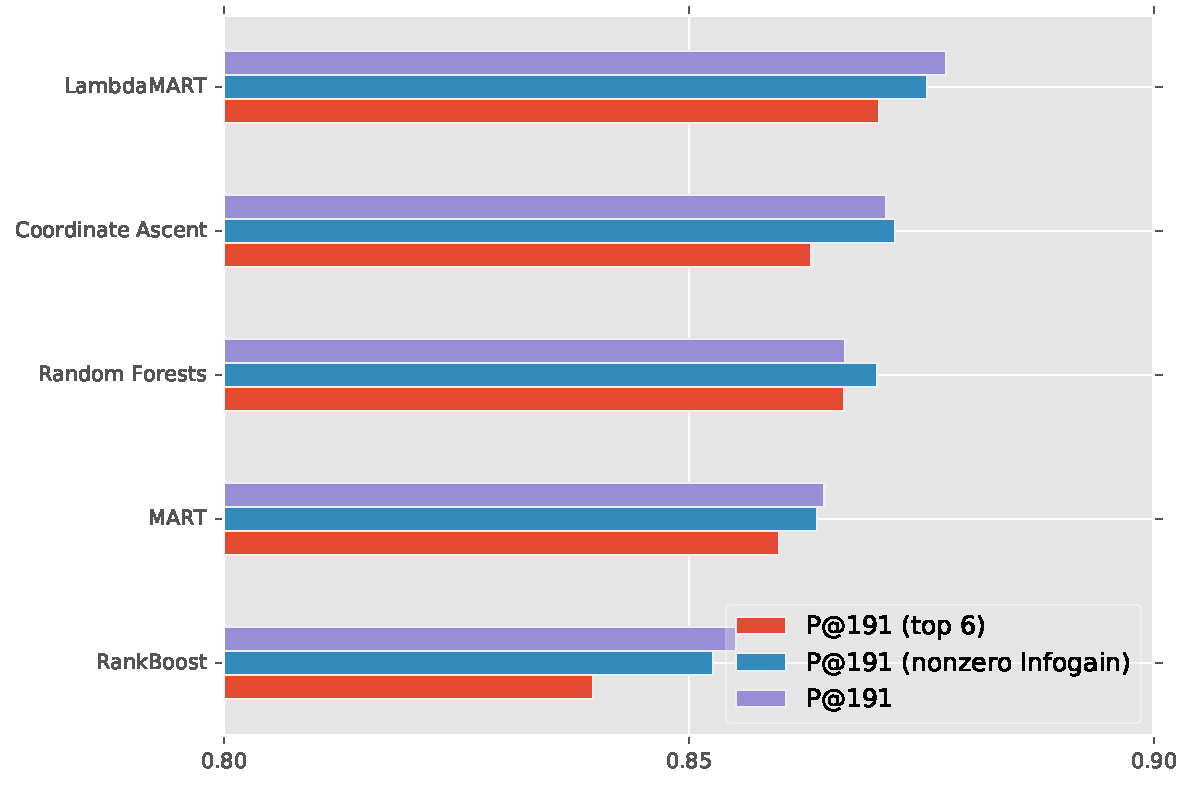
\includegraphics[width=\linewidth]{images/results_p191}
  \end{figure}
\end{frame}

\begin{frame}
  \frametitle{Results for PP@75}
  \begin{figure}[tbph]
    \centering
    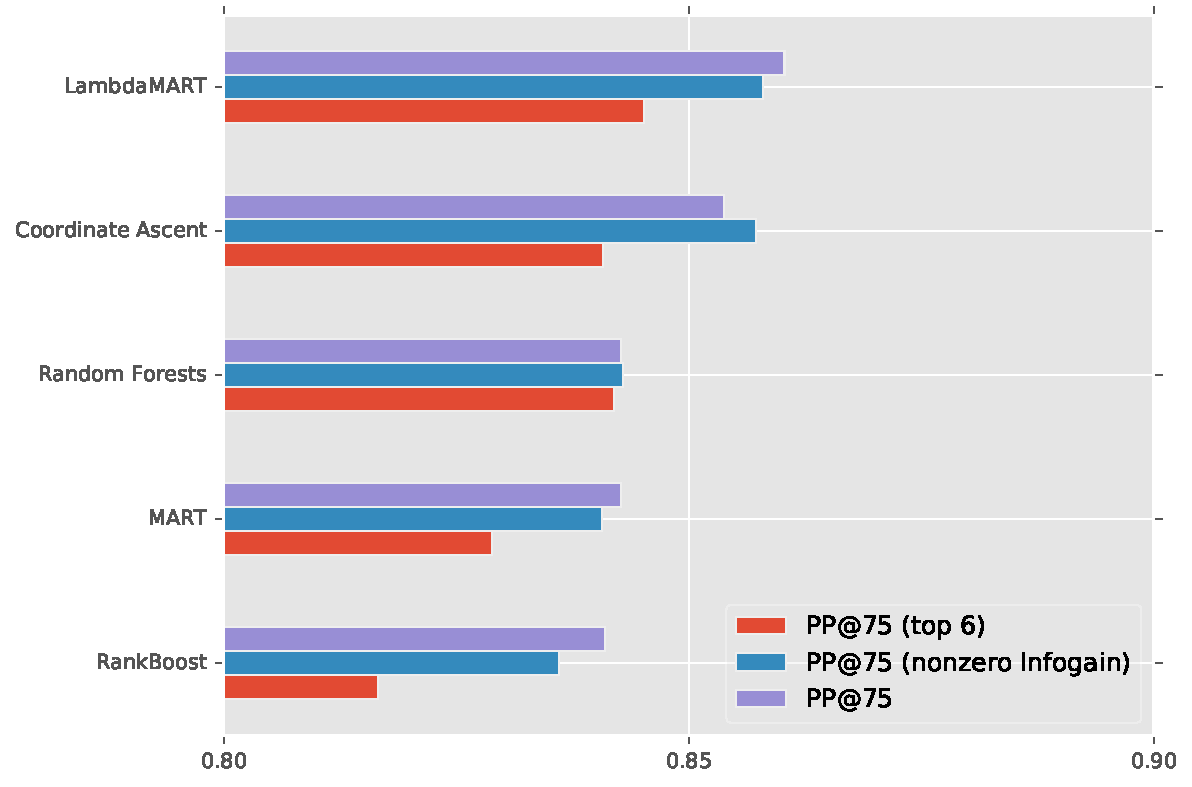
\includegraphics[width=\linewidth]{images/results_pp75}
  \end{figure}
\end{frame}

\begin{frame}
  \frametitle{Results for PP@50}
  \begin{figure}[tbph]
    \centering
    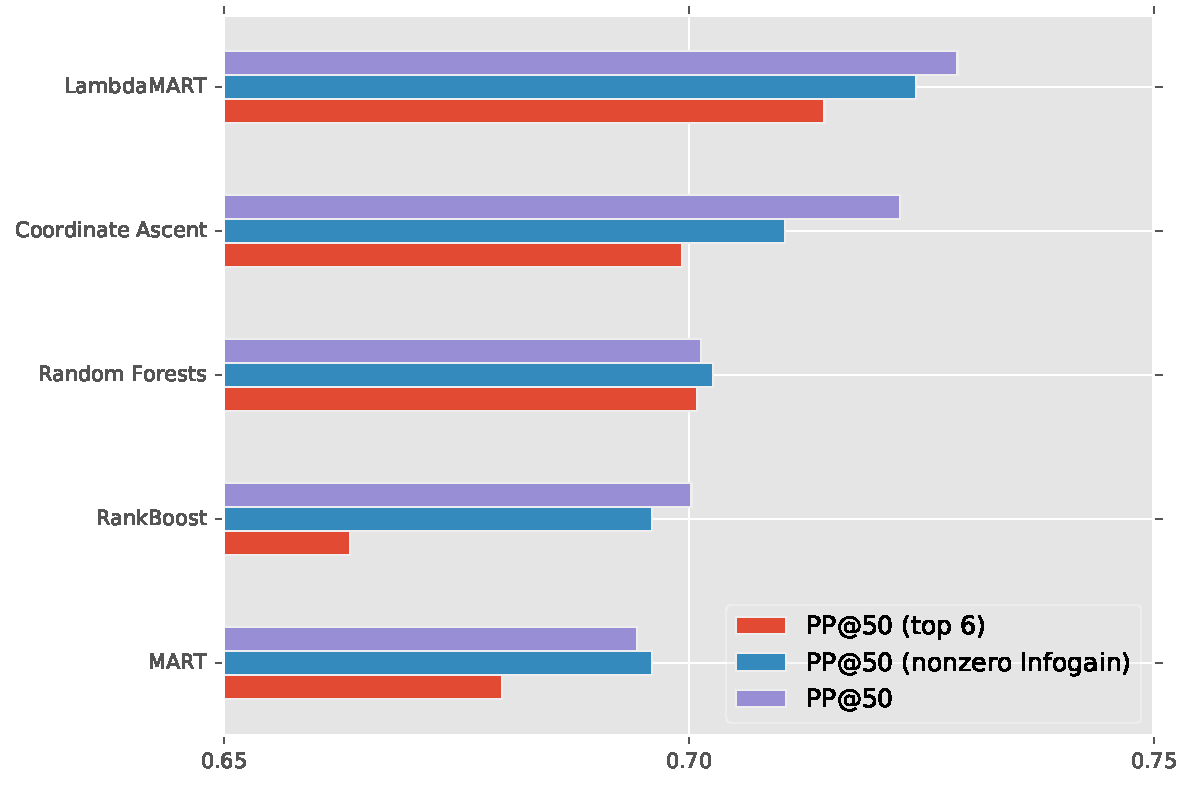
\includegraphics[width=\linewidth]{images/results_pp50}
  \end{figure}
\end{frame}

\begin{frame}
  \frametitle{Results for PP@k for various k}
  \begin{figure}[tbph]
    \centering
    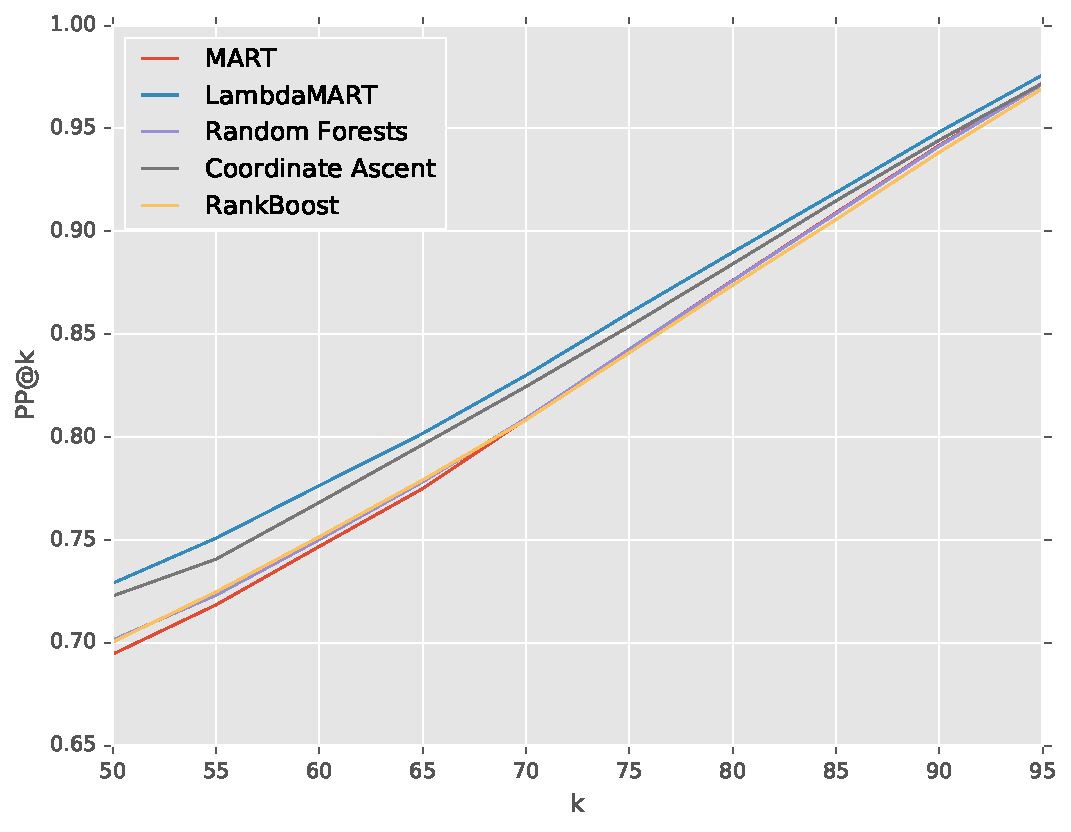
\includegraphics[width=0.95\linewidth]{images/results_pp_k}
  \end{figure}
\end{frame}

\begin{frame}
  \frametitle{Comparison of learning times}
  \begin{figure}[tbph]
    \centering
    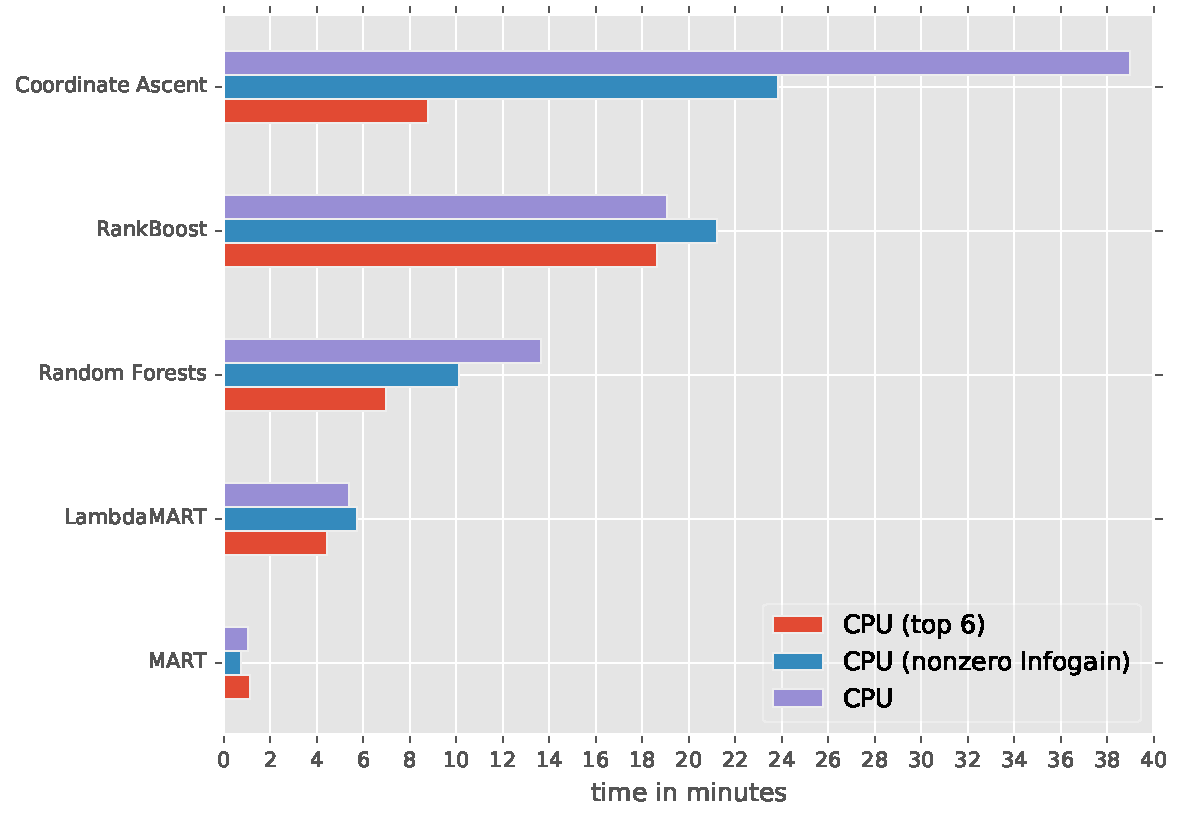
\includegraphics[width=0.95\linewidth]{images/results_times}
  \end{figure}
\end{frame}

%------------------------------------------------

\section{Discussion}

\paragraph{Feature Selection}
Reasons for feature selection are to reduce overfitting and eliminate possible truly redundant features -- moreover, reducing the number of features can simplify the model and make it easier to interpret. In this work we focused mainly on potential performance benefits, but the results from table \ref{tab:feature_relevance} can also be useful for identifying feature subsets with potential to outperform full set. For example, taking only features with non-zero Infogain is one possible approach.
% * <philip@thruesen.dk> 2016-06-01T19:00:00.702Z:
%
% outcommented a paragraph. I dont believe using a subset of features will ever perform better than the full set unless there's overfitting which I think is very unlikely for our model.
%
% ^ <jarekcechak@gmail.com> 2016-06-02T09:10:39.850Z:
%
% This is what Nattiya told us that feature selection is usually used for
%
% ^ <jarekcechak@gmail.com> 2016-06-02T09:10:44.022Z.
% * <philip@thruesen.dk> 2016-06-01T18:56:01.192Z:
%
% > truly redundant
%
% changed conflicting to truly redundant. Change back if you disagree
%
% ^ <roelcastanomoreno@gmail.com> 2016-06-02T09:12:22.872Z.

All three methods used to evaluate the features are only heuristics and don't completely reflect true value of features. They are mainly focused on isolated importance of single feature, there might be however, complex relations between some features that will not be identified this way.

\paragraph{Applicability of Model. }
It is interesting to discuss the realistic applicability of the models generated by this research. We realize that having a fixed threshold for the number of links that may appear in an article is a na\"{\i}ve solution to the problem of overlinking. The correct number of links that may appear in an article should rather be determined by some function that considers the length of the article. Computing this is outside the scope of this work and any limits are best to be defined by Wikipedia policy makers. Depending on the use case of the suggested model, the degree to which the feature selection is needed can be reconsidered, i.e. how many resources to dedicate to the training and use of such a model.
%With that in mind and some possible improvements (Choosing a correct threshold for the number or percentage of links), 
Summarizing these thoughts, we think the model applies well to Wikipedia articles and possibly other wiki-based sites. There's always a risk that some articles `lose' a small percentage of useful links if the model was used with full automation but the benefits of improving readability through Wikipedia might out-weight the drawbacks. It may also simply be used as a tool for editors, alerting them when they are about to add a link that might confuse future readers more than it would help them.

\paragraph{Future Work}
Naturally, it is possible to expand the work done in this article. Many aspects of the research were limited by significant restraints on processing power and time availability. If more resources were available the project could be extended and up-scaled in multiple obvious ways.%, but it can be easily extended by building upon the different components.

For the future, one might choose to increase amount of articles in the dataset and change the strategy with which they are selected.  For this article, we chose the 1000 articles having the most outgoing clicks. In this way we were sure to have only articles where a ranking of referred articles was possible. Had we e.g. included articles in the prominent set without outgoing clicks we would have to rank a set of referred articles all assigned to the same label (of zero). %Another strategy to select prominent articles might be to choose one or multiple clusters of articles to generate the model or a random sample.

There's much work that could be done for the set of features. E.g. the features describing link position could be supplemented with the link position based on the visual representation after HTML had been rendered. Moreover, some features describing explicit categories could be added and the 'generality' of an article, which represents how specific or general the topic discussed is (to the general public). We have skipped construction of some potential features like the ones mentioned above due to prioritization considering our limited time.

Finally, another possibility is to evaluate other implementations of Learning to Rank algorithms or modify the existing ones. This was also outside of the scope of the project. 

%----------------------------------------------------------------------------------------
%	REFERENCE LIST
%----------------------------------------------------------------------------------------

\begin{thebibliography}{99} % Bibliography - this is intentionally simple in this template
	
	\bibitem[1]{learning_link}
	D. Milne and I. H. Witten,
	\newblock "Learning to Link with Wikipedia"
	\newblock \emph{ Proceeding of the 17th ACM Conference on Information and Knowledge Mining - CIKM '08 (2008): Web.}
	
	\bibitem[2]{west}
	R. West, A. Paranjape, and J. Leskovec,
	\newblock "Mining Missing Hyperlinks from Human Navigation Traces: A Case Study of Wikipedia"
	\newblock \emph{Proceedings of the 24th International Conference on World Wide Web - WWW '15 (2015): Web}
		
	\bibitem[3]{paranjape}
	A. Paranjape, R. West, L. Zia, and J. Leskovec,
	\newblock "Improving Website Hyperlink Structure Using Server Logs"
	\newblock \emph{Proceedings of the Ninth ACM International Conference on Web Search and Data Mining - WSDM '16 (2016): Web}

	\bibitem[4]{li}
	H. Li,
	\newblock "A Short Introduction to Learning to Rank"
	\newblock \emph{IEICE Transactions on Information and Systems IEICE Trans. Inf. \& Syst. E94-D.10 (2011): 1854-862}
	
	\bibitem[5]{nielsen}
	J. Nielsen,
	\newblock "How Users Read on the Web"
	\newblock \emph{Nielsen Norman Group. N.p., n.d. Web. 6 May 2008}

	\bibitem[6]{lead}
	"Lead Section"
	\newblock \emph{Wikipedia. Wikimedia Foundation.}
	\newblock https://en.wikipedia.org/wiki/ \\ Wikipedia:Manual\_of\_Style/Lead\_section
	
\end{thebibliography}


%----------------------------------------------------------------------------------------

\end{multicols}

\end{document}
